\hypertarget{algebraic-and-number-theoretic-basics}{%
\section{Algebraic and Number Theoretic Basics}\label{algebraic-and-number-theoretic-basics}}

\hypertarget{division-theorem}{%
\subsection{Division Theorem}\label{division-theorem}}

If $a$ is not 0, then $a$ can divide $n$, if there is a number $b$, that is true
for $n = a * b$.
If $a$ and $b$ are integers with $b$ \textgreater{} $0$ then there are unique
integers $q$ and $r$ such that $a = q*b+r$ and $0 <= r < b$

\begin{tcolorbox}[colback=red!5!white,colframe=red!75!black]
    Heisst nichts anderes, $a$ ist durch $b$ teilbar, ergibt einen Quotienten $b$ und einen Rest $r$.
\end{tcolorbox}

\hypertarget{greatest-common-divisor-gcd}{%
\subsection{Greatest Common Divisor
(gcd)}\label{greatest-common-divisor-gcd}}

Largest non-negative integer $d$ that divides both $a$ and $b$

\begin{tcolorbox}[colback=red!5!white,colframe=red!75!black]
    Special case: gcd(0,0) = 0 
\end{tcolorbox}

1 ist immer eine Zahl der gemeinsamen Teiler. Die gemeinsamen Teiler sind nach oben beschränkt, da ist dann der grösste gemeinsame Teiler. \textbf{Teilerfremd} bedeutet, wenn zwei Zahlen nur durch 1 teilbar sind.

\begin{itemize}
\tightlist
\item
  gcd(a,0) = \textbar{}a\textbar{} (also valid for a = 0)
\item
  Wenn ich a um ein Vielfaches von b addiere, ist der gcd immer noch der
  gcd von a \& b. also
\item
  Resultiert: gcd(a+q*b,b) = gcd(a,b)
\item
  \textbf{gcd(a mod b, b) = gcd(a,b)}
\end{itemize}

\hypertarget{euclid-algorithm}{%
\subsection{Euclid Algorithm}\label{euclid-algorithm}}

\begin{tcolorbox}[colback=red!5!white,colframe=red!75!black]
\bf{gcd(a, b):} \\
$while (a!=0): \\ 
  r = b \mod a \\
  b = a  \\
  a = r \\
return = b$ 
\end{tcolorbox}

\hypertarget{extended-euclid-algorithm}{%
\subsection{Extended Euclid Algorithm}\label{extended-euclid-algorithm}}

For any given integers $a, b, n$ the equation \textbf{$a*x + b*y = n$} can be solved by integers $x$ and $y$ \textbf{if and only if gcd(a,b)\textbar{}n}. \emph{x and y don't have to be unique. The result is just a possible one.}

\begin{tcolorbox}[colback=red!5!white,colframe=red!75!black]
function [ gcd, x, y ] = egcd(a, b)\\
\textit{Input: Integers a, b} \\
\textit{Output: gcd(a,b) and x,y with ax + by = gcd(a,b)} \\
$x = 0; \\
y = 1; \\
u = 1; \\
v = 0; \\
while a \neq 0 \\
    q = floor(b/a);$ integer divison  \\
    $r = \mod(b,a); \\
    m = x - u*q; \\
    n = y - v*q; \\
    b = a; \\
    a = r; \\
    x = u; \\
    y = v; \\
    u = m; \\
    v = n; \\
end \\
gcd = b;$ \\
end
\end{tcolorbox}

\begin{figure}[H]
\centering
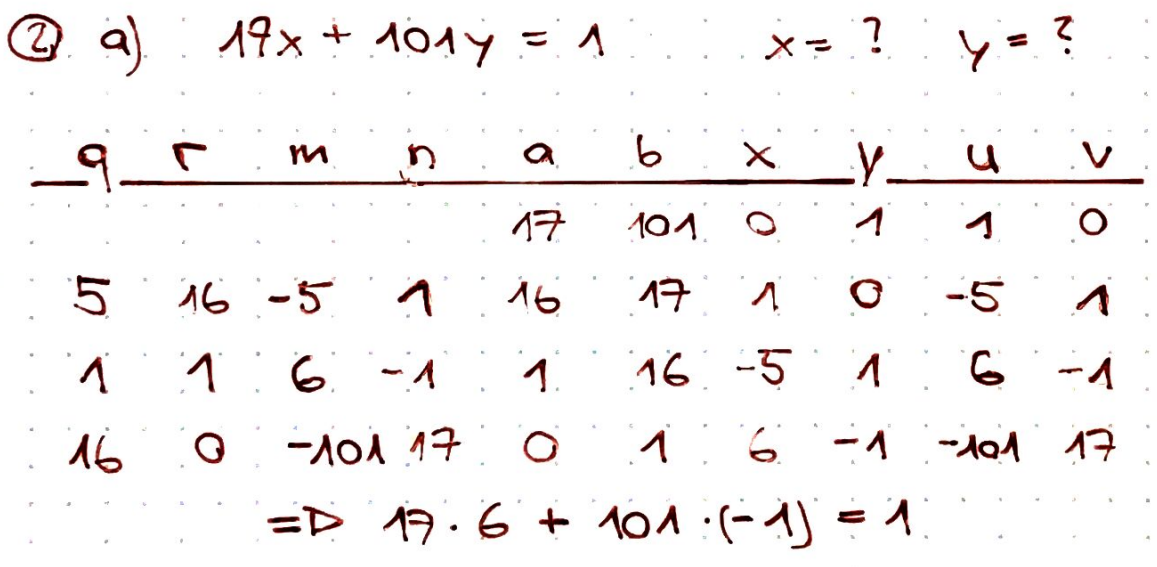
\includegraphics[width=1\textwidth]{figures/extendedEuclidAlgorithm.png}
\caption{Extended Euclid Algorithm}
\end{figure}

\hypertarget{modulo}{%
\subsection{Modulo}\label{modulo}}

$3, 27, 51 \mod 24$ sind kongruent. Geschrieben wird dies \textbf{$a \equiv b \mod n$} -> a ist kongruent zu b Modulo n.

\hypertarget{eigenschaften}{%
\subsubsection{Eigenschaften}\label{eigenschaften}}

\begin{itemize}
\tightlist
\item
  z.B. a = 17, b = 23, n = 3. Die sind kongruent Modulo 3
\item
  Die Differenz von a und b ist durch n teilbar, ohne Rest
\item
  Zudem a = b + n*k (a ist gleich b plus ein Vielfaches von n)
\end{itemize}

Alle Zahlen, die bei Division durch 16 denselben Rest ergeben, nennt man
eine \textbf{Kongruenzklasse} Modulo 16.

\hypertarget{inverse-kehrwert}{%
\subsection{Inverse (Kehrwert)}\label{inverse-kehrwert}}

Ein \textbf{Kehrwert} beschreibt diejenige Zahl, die mit x multipliziert
die Zahl 1 ergibt.

\hypertarget{modular-inverses}{%
\subsubsection{Modular Inverses}\label{modular-inverses}}

If the congruence a*x $\equiv{1} \mod{n}$ has a solution, we say a is invertible
modulo n or Modular Inverse (\textbf{if gcd(a,n) = 1}).

The modular multiplicative inverse of an integer a modulo m is an integer b such that
$a*b \equiv 1 \mod m$,
e.g. $2*4  \equiv 1 \mod 7$ (4 is the Modular Multiplicative Inverse of 2 mod 7)

\begin{tcolorbox}[colback=red!5!white,colframe=red!75!black]
Um den Modular Inverse zu ermitteln, kann auch der erweiterte euklidische Algorithmus angewendet werden:
$1 = ax + my$

Wenn man daran bereits jetzt den Modulo m anwendet, sieht man dass x das Modulo Inverse von a Mod m ist:
$1 = ax + m \mod m$

Für a = 5 und m = 12 ergibt das mit dem erweiterten euklidischen Algorithmus x = 5, was in der Tat ein modularer Kehrwert von $\mod 12$ ist:
$5 * 5 = 25 \equiv 1 \mod 12.$
\end{tcolorbox}

\hypertarget{fermats-little-theorem}{%
\subsection{Fermat's Little Theorem}\label{fermats-little-theorem}}

If p is a prime and p does not divide a, then

\begin{tcolorbox}[colback=red!5!white,colframe=red!75!black]
$a^p \equiv a \mod p$
\end{tcolorbox}

\textbf{If a and p are coprime} (if there is a modular inverse), one can
cancel a factor a and one gets

\begin{tcolorbox}[colback=red!5!white,colframe=red!75!black]
$a^{(p-1)} \equiv 1 \mod p$
\end{tcolorbox}

\hypertarget{eulers-phi-function}{%
\subsection{Euler's Phi-Function}\label{eulers-phi-function}}

Ich habe irgendeine ganze Zahl n. Ich frage mich, zwischen 1 und n, gibt
es gewisse Zahlen die sind teilerfremd zu n, und es gibt gewisse Zahlen
die sind nicht teilerfremd zu n. Die eulersche Phi-Funktion ergibt das
Resultat der \textbf{Anzahl teilerfremden Zahlen von 1 zu n}.

\begin{tcolorbox}[colback=red!5!white,colframe=red!75!black]
Relativley prime, coprime oder teilerfremd bedeutet alles dasselbe. \\
y(n) = numbers of integers 1 <= a <= n such that gcd(a,n) = 1
\end{tcolorbox}

\begin{tcolorbox}[colback=red!5!white,colframe=red!75!black]
Wenn p eine Primzahl ist, ist y(p) = p-1 

Wenn p und q zwei ungleiche Primzahlen sind, ist $y(p*q) = p * q - q - p + 1 = (p-1)(q-1)$

$y(p^n) = p^n - p^{(n-1)} = p^{n-1} *(p-1)$

Wenn gcd(m,n)=1, dann kann man $y(m * n) = y(m) * y(n)$ rechnen
\end{tcolorbox}

\hypertarget{primzahlzerlegung}{%
\subsubsection{Primzahlzerlegung}\label{primzahlzerlegung}}

Für jede Zahl n gibt es eine Primzahlzerlegung. Dies kann man für jede
Zahl machen, die selbst keine Primzahl ist. z.B. 8 ist 2 * 2 * 2.

\begin{figure}[H]
\centering
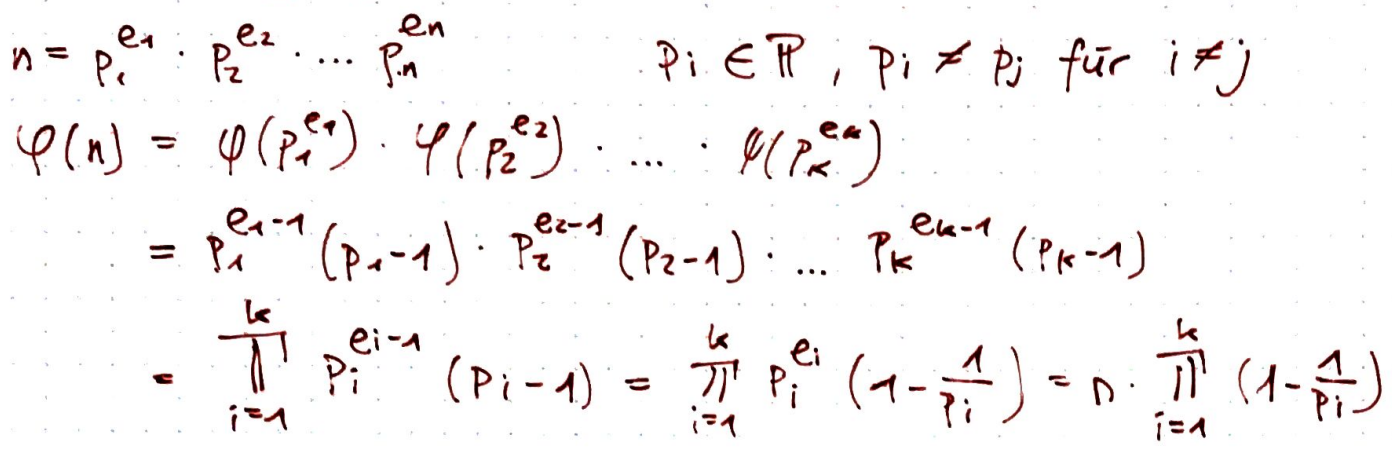
\includegraphics[width=1\textwidth]{figures/primzahlZerlegung.png}
\caption{Primzahlzerlegung}
\end{figure}

\begin{tcolorbox}[colback=red!5!white,colframe=red!75!black]
Es ist von identischer Schwierigkeit, das Phi von n zu berechnen, wie die Primfaktorzerlegung von der Zahl n zu machen.
\end{tcolorbox}

\hypertarget{eulers-totient-theorem}{%
\subsection{Euler's Totient Theorem}\label{eulers-totient-theorem}}

Eulers Vereinfachung von Fermat's Theoreom.

\begin{figure}[H]
\centering
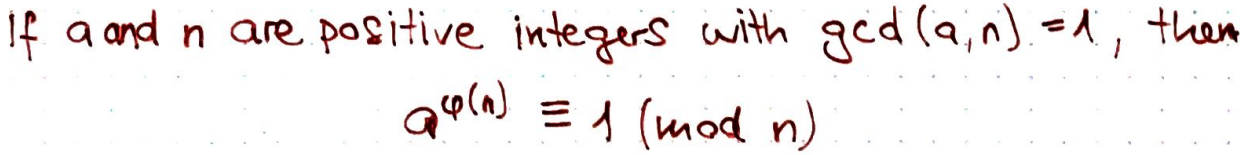
\includegraphics[width=0.6\textwidth]{figures/eulersTotientTheorem.png}
\caption{Euler's Totient Theorem}
\end{figure}

\hypertarget{multiplikative-ordnung}{%
\subsection{Multiplikative Ordnung}\label{multiplikative-ordnung}}

Die Multiplikative Ordnung von g modulo n ist die kleinst möglich
positive Zahl e so dass $g^e \equiv 1 \mod n$ ist.

\begin{tcolorbox}[colback=red!5!white,colframe=red!75!black]
$g^f \equiv 1 \mod n$ ist dann möglich, wenn $f$ durch die multiplikative Ordnung $e$ teilbar ist. 
e.g. wenn $ord(2) = 4$, dann kann f z.B. 8 oder 12 sein.

Angenommen $g^e \equiv 1 \mod n$. Es gilt $g^k \equiv g^l \mod n$ nur dann, wenn $k \equiv l \mod e$

Wenn $e$ die multiplikative Ordnung von $g$ ist, dann ist $g^k \equiv e / gcd(e, k)$.
\end{tcolorbox}

\begin{figure}[H]
\centering
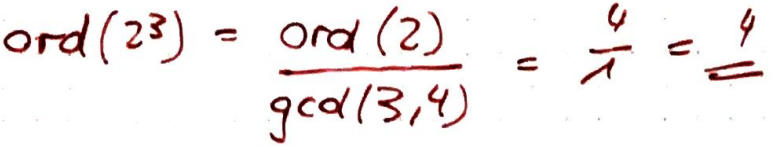
\includegraphics[width=1\textwidth]{figures/multiplicativeOrderExample.png}
\caption{Beispiel Multiplikative Ordnung}
\end{figure}

\hypertarget{generator-modulo-p}{%
\subsection{Generator modulo p}\label{generator-modulo-p}}

Ein Zahl a zwischen 1 und p-1 ist ein generierendes Element, wenn es durch
potentieren ($a^0$,$a^1$, \ldots{}) $\mod$ p alle Zahlen zwischen 1 bis
p generiert.

\begin{tcolorbox}[colback=red!5!white,colframe=red!75!black]
Egal welche Primzahl gewählt wird, es gibt immer mindestens ein Generator Element
\end{tcolorbox}

\begin{figure}[H]
\centering
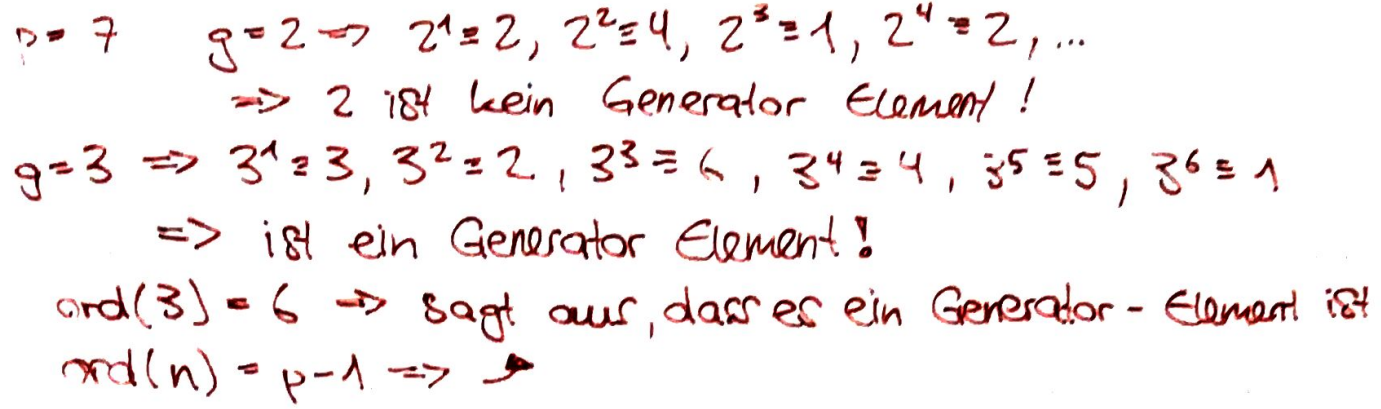
\includegraphics[width=1\textwidth]{figures/generatorElementExample.png}
\caption{Generator Element}
\end{figure}

\clearpage
\hypertarget{chinese-remainder-theorem}{%
\subsection{Chinese Remainder Theorem}\label{chinese-remainder-theorem}}

Wir suchen ein Grösse x, von der wir wissen\\
$x \equiv a1 \mod m1$\\
\ldots{}\\
$x \equiv an (mod mn)$\\
\emph{(System von simultanen Kongruenzen)}

\begin{figure}[H]
\centering
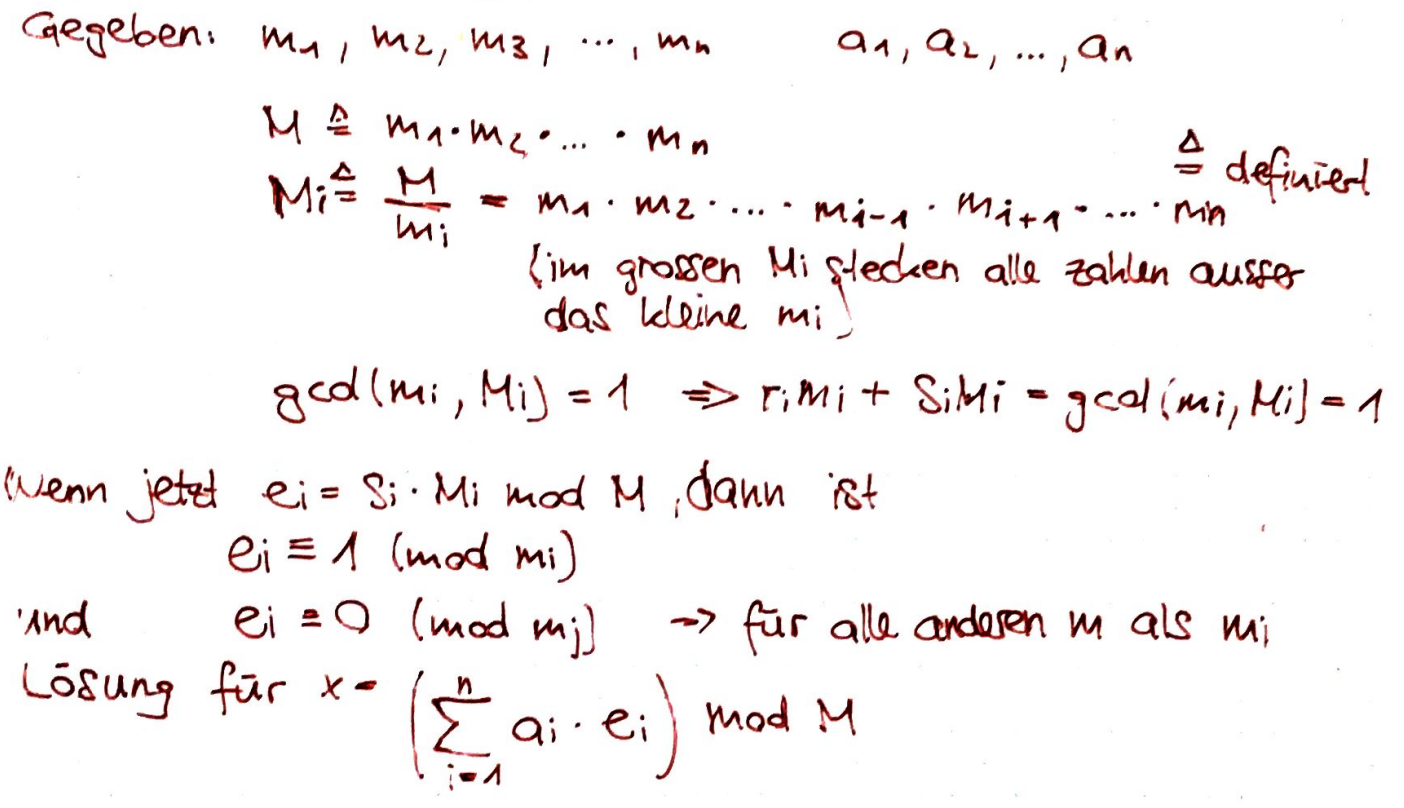
\includegraphics[width=0.8\textwidth]{figures/chinesischerRestsatz.png}
\caption{Chinese Remainder Theorem}
\end{figure}

\begin{figure}[H]
\centering
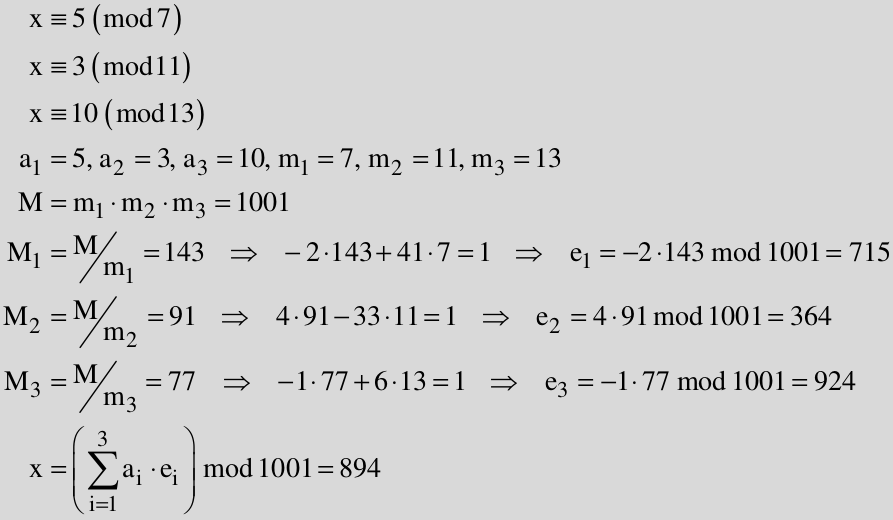
\includegraphics[width=0.8\textwidth]{figures/chinesischerRestsatzExample.png}
\caption{Chinese Remainder Theorem - Example}
\end{figure}

\clearpage
